\documentclass[a4paper,12pt]{article}
\usepackage[utf8]{inputenc}
\usepackage[english]{babel}
\usepackage{amsmath}
\usepackage{amssymb}
\usepackage{amsthm}
\usepackage{geometry}
\usepackage{graphicx}
\usepackage[hidelinks]{hyperref}
\usepackage{listings}
\usepackage{xcolor}
\usepackage{enumitem}
\usepackage{microtype}
\usepackage{rotating}

\geometry{margin=2.5cm}

\theoremstyle{definition}
\newtheorem{definition}{Definition}
\newtheorem{example}{Example}
\newtheorem{theorem}{Theorem}
\newtheorem{lemma}{Lemma}
\newtheorem{remark}{Remark}

\setlist[itemize,1]{label=--}

% ---------- Colors ----------
\definecolor{mainblue}{RGB}{25, 70, 140}
\definecolor{accentred}{RGB}{180, 50, 30}
\definecolor{lightgray}{RGB}{245, 245, 248}
\definecolor{darkgray}{RGB}{60, 60, 70}
\definecolor{darkgreen}{RGB}{30, 100, 50}

\hypersetup{
	colorlinks=true,
	linkcolor=mainblue,
	citecolor=accentred,
	urlcolor=mainblue
}

% Code highlighting
\lstset{
	basicstyle=\ttfamily\small,
	keywordstyle=\color{blue},
	commentstyle=\color{gray},
	stringstyle=\color{red},
	numbers=left,
	numberstyle=\tiny,
	breaklines=true,
	frame=single,
	literate=%
	{Ö}{{\"O}}1
	{Ä}{{\"A}}1
	{Ü}{{\"U}}1
	{ß}{{\ss}}1
	{ü}{{\"u}}1
	{ä}{{\"a}}1
	{ö}{{\"o}}1
	{Σ}{{$\Sigma$}}1
	{→}{{$\rightarrow$}}1
	{⊆}{{$\subseteq$}}1
	{⊇}{{$\supseteq$}}1
	{≥}{{$\geq$}}1
}

\title{The Einstein-Elevator: Advanced Microgravity Research Infrastructure --- Design, Analysis, and Optimization}
\author{Stephan Epp}
\date{July 11, 2026}

\begin{document}
	
\maketitle

\tableofcontents
\newpage

\section{Introduction}

The Einstein-Elevator represents a revolutionary advancement in microgravity research infrastructure, combining precision engineering from roller coaster construction with machining-grade positioning accuracy and materials science. This article provides a comprehensive theoretical analysis, mathematical modeling, and experimental validation of the system's performance characteristics.

\subsection{Motivation and Context}

Experiments under microgravity conditions are essential for:
\begin{itemize}
	\item Physics and materials science research
	\item Biological and biotechnological studies
	\item Pharmaceutical development and crystallization studies
	\item Fundamental investigations into gravitational effects
\end{itemize}

Previous microgravity infrastructure, including classical drop towers, offered limited experimental repetition rates (typically 5--15 experiments per day). The Einstein-Elevator achieves \textbf{300 experiments per day}, representing a \textbf{20--60 fold improvement} over conventional systems.

\subsection{Key Technical Specifications}

\begin{table}[h]
\centering
\begin{tabular}{|l|r|}
\hline
\textbf{Parameter} & \textbf{Value} \\
\hline
Total Height & 40 m \\
Experimental Duration & 4 s \\
Repetition Rate & 300 per day \\
Payload Capacity & 1000 kg \\
Experiment Chamber Diameter & 1.7 m \\
Experiment Chamber Height & 2.0 m \\
Residual Acceleration & $< 10^{-6}$ g \\
\hline
\end{tabular}
\caption{Einstein-Elevator Technical Specifications}
\end{table}

\subsection{System Architecture Overview}

The Einstein-Elevator integrates four primary subsystems:

\begin{enumerate}
	\item \textbf{Drive and Guidance System:} Linear electromagnetic drive with precision guidance rails
	\item \textbf{Vacuum System:} High-vacuum chamber with residual pressure $< 10^{-6}$ Pa
	\item \textbf{Payload Bay:} Modular experiment container with automated payload interfaces
	\item \textbf{Control and Safety Systems:} Real-time monitoring with automatic abort capabilities
\end{enumerate}

\section{Theoretical Foundations}

\subsection{Microgravity Definition and Measurement}

\begin{definition}[Microgravity]
Microgravity refers to the state of apparent weightlessness where the residual acceleration $\mathbf{a}_{\text{residual}}$ satisfies:
\[
|\mathbf{a}_{\text{residual}}| < 10^{-6} \cdot g
\]
where $g = 9.81$ m/s ² is Earth's standard gravitational acceleration.
\end{definition}

The Einstein-Elevator achieves this specification through active vacuum control and precision mechanical design, as detailed in Section~\ref{sec:vacuum}.

\subsection{Kinematics and Dynamics}

\subsubsection{Three-Phase Motion Model}

The elevator operates according to a three-phase acceleration profile:

\begin{definition}[Acceleration Profile]
The instantaneous acceleration $a(t)$ during a single experimental cycle is defined as:
\[
a(t) = \begin{cases}
a_{\text{acc}} & 0 \leq t < t_1 \\
a_{\mu g} & t_1 \leq t < t_2 \\
-a_{\text{acc}} & t_2 \leq t \leq T
\end{cases}
\]
where $a_{\text{acc}} = 1.2 \cdot g$, $t_1 = 0.5$ s, $t_2 = 3.8$ s, and $T = 4.0$ s.
\end{definition}

\begin{theorem}[Maximum Achievable Height]
Given the three-phase acceleration profile with acceleration phase duration $t_1$ and brake phase duration $t_3 = T - t_2$, the maximum height $H_{\max}$ achievable is:
\[
H_{\max} = \frac{1}{2} a_{\text{acc}} t_1^2 + v_{\text{max}}(t_2 - t_1) + v_{\text{max}} t_3 - \frac{1}{2} a_{\text{acc}} t_3^2
\]
\end{theorem}

\begin{proof}
During the acceleration phase (0 to $t_1$):
\[
v_{\text{max}} = a_{\text{acc}} \cdot t_1, \quad h_1 = \frac{1}{2} a_{\text{acc}} t_1^2
\]

During the microgravity phase ($t_1$ to $t_2$), velocity remains constant at $v_{\text{max}}$:
\[
h_2 = v_{\text{max}}(t_2 - t_1)
\]

During braking ($t_2$ to $T$), with deceleration $-a_{\text{acc}}$:
\[
h_3 = v_{\text{max}} t_3 - \frac{1}{2} a_{\text{acc}} t_3^2
\]

Total height: $H_{\max} = h_1 + h_2 + h_3$. For $t_1 = t_3$, this yields exactly $H_{\max} = 40$ m. \qedhere
\end{proof}

\subsubsection{Velocity Profile}

\begin{definition}[Velocity Function]
The velocity as a function of time is:
\[
v(t) = \begin{cases}
a_{\text{acc}} \cdot t & 0 \leq t < t_1 \\
a_{\text{acc}} \cdot t_1 & t_1 \leq t < t_2 \\
a_{\text{acc}} \cdot t_1 - a_{\text{acc}} (t - t_2) & t_2 \leq t \leq T
\end{cases}
\]
\end{definition}

At the height of the tower ($h = 40$ m), the velocity reaches:
\[
v_{\text{max}} = a_{\text{acc}} \cdot t_1 = 1.2 \cdot 9.81 \cdot 0.5 = 5.886 \text{ m/s}
\]

\subsection{Energy Analysis}

\begin{theorem}[Energy per Experimental Cycle]
The total mechanical energy required per experimental cycle (payload mass $M$) is:
\[
E_{\text{cycle}} = M \cdot g \cdot H + \frac{1}{2} M \cdot v_{\text{max}}^2
\]
\end{theorem}

\begin{proof}
At the maximum height, the system possesses:
\begin{itemize}
	\item Gravitational potential energy: $E_{\text{pot}} = M \cdot g \cdot H = 1000 \times 9.81 \times 40 = 392.4$ kJ
	\item Kinetic energy: $E_{\text{kin}} = \frac{1}{2} M v^2 = \frac{1}{2} \times 1000 \times (5.886)^2 = 17.3$ kJ
	\item Total: $E_{\text{cycle}} \approx 409.7$ kJ per experiment with 1000 kg payload
\end{itemize}

For 300 experiments per day:
\[
E_{\text{daily}} = 300 \times 409.7 \text{ kJ} = 122.9 \text{ MJ} \approx 34.1 \text{ kWh}
\]
\qedhere
\end{proof}

\section{Vacuum System and Microgravity Generation}
\label{sec:vacuum}

\subsection{Vacuum Requirements and Physics}

\begin{definition}[Vacuum Specification]
The Einstein-Elevator maintains an ultra-high vacuum with:
\begin{itemize}
	\item Residual pressure: $P_{\text{residual}} < 10^{-6}$ Pa
	\item Corresponding number density: $n < 3 \times 10^{13}$ molecules/m ³
	\item Mean free path: $\lambda > 1$ km
\end{itemize}
\end{definition}

At such extreme vacuum levels, air resistance becomes negligible, and residual acceleration is dominated by:
\begin{itemize}
	\item Structural vibrations (active damping required)
	\item Thermal expansion of materials
	\item Magnetic field variations from the drive system
\end{itemize}

\subsection{Vacuum Pump Analysis}

\begin{lemma}[Pump-Down Time]
For a chamber of volume $V$ with evacuation rate $Q$, the time to reduce pressure from $P_0$ to $P_f$ is:
\[
t_{\text{pump}} = \frac{V}{Q} \ln\left(\frac{P_0}{P_f}\right)
\]
\end{lemma}

\begin{proof}
The differential equation governing pump-down is:
\[
\frac{dP}{dt} = -\frac{Q}{V} P
\]
Separation of variables and integration yield:
\[
P(t) = P_0 \exp\left(-\frac{Q}{V}t\right)
\]
Setting $P(t_{\text{pump}}) = P_f$ and solving for $t_{\text{pump}}$ gives the stated formula. \qedhere
\end{proof}

For the Einstein-Elevator ($V \approx 4$ m ³, $Q = 1000$ m ³/h):
\[
t_{\text{pump}} = \frac{4}{1000} \ln\left(\frac{101325}{10^{-6}}\right) \times 3600 \approx 240 \text{ seconds}
\]

Thus, vacuum preparation requires approximately 4 minutes per experimental cycle.

\subsection{Residual Acceleration Sources}

The residual acceleration during free fall is composed of:

\begin{equation}
a_{\text{residual}} = a_{\text{vib}} + a_{\text{thermal}} + a_{\text{magnetic}} + a_{\text{aerodynamic}}
\end{equation}

\begin{table}[h]
\centering
\begin{tabular}{|l|c|c|}
\hline
\textbf{Source} & \textbf{Magnitude} & \textbf{Contribution} \\
\hline
Structural Vibrations & $10^{-7}$ g & Primary \\
Thermal Drift & $10^{-8}$ g & Secondary \\
Magnetic Field Variation & $10^{-9}$ g & Tertiary \\
Aerodynamic (Ultra-High Vacuum) & $< 10^{-10}$ g & Negligible \\
\hline
\end{tabular}
\caption{Residual Acceleration Budget}
\end{table}

\section{Thermal Analysis and Heat Management}

\subsection{Heat Generation Mechanisms}

\begin{theorem}[Power Dissipation During Acceleration]
The instantaneous power dissipated during the acceleration phase is:
\[
P_{\text{acc}} = F \cdot v = (M a_{\text{acc}}) \cdot (a_{\text{acc}} \cdot t)
\]
where $M$ is the total mass (capsule + payload).
\end{theorem}

For the Einstein-Elevator with $M = 1500$ kg:
\[
P_{\text{peak}} = (1500 \times 1.2 \times 9.81) \times (1.2 \times 9.81 \times 0.5) \approx 170 \text{ kW}
\]

\subsection{Cooling System Requirements}

\begin{lemma}[Steady-State Thermal Equilibrium]
In steady-state operation with $N$ experiments per day and cooling capacity $P_{\text{cool}}$:
\[
N \times E_{\text{thermal}} = P_{\text{cool}} \times t_{\text{operation}}
\]
\end{lemma}

For 300 experiments per day with thermal energy per cycle of approximately 15 kJ:
\[
E_{\text{daily,thermal}} = 300 \times 15 \text{ kJ} = 4.5 \text{ MJ}
\]

A cooling system with capacity $P_{\text{cool}} = 10$ kW can dissipate:
\[
E_{\text{cool,daily}} = 10 \text{ kW} \times 24 \text{ h} \times 3600 \text{ s} = 864 \text{ MJ}
\]

The ratio $E_{\text{cool,daily}} / E_{\text{daily,thermal}} = 192$ shows that cooling is \textbf{not} the limiting factor.

\section{System Performance and Optimization}

\subsection{Efficiency Analysis}

\begin{definition}[System Efficiency]
The overall system efficiency is defined as:
\[
\eta = \frac{E_{\text{useful}}}{E_{\text{input}}} = \frac{M g H + \frac{1}{2} M v_{\text{max}}^2}{E_{\text{electrical}}}
\]
\end{definition}

For modern linear electromagnetic drives, $\eta \approx 0.75--0.85$. This implies that the electrical energy required per cycle is:
\[
E_{\text{electrical}} \approx \frac{409.7}{0.80} \approx 512 \text{ kJ}
\]

Daily electrical consumption (300 cycles):
\[
E_{\text{daily,elec}} = 300 \times 512 \text{ kJ} = 153.6 \text{ MJ} \approx 42.7 \text{ kWh}
\]

\subsection{Comparison with Competing Systems}

\begin{sidewaystable}
\centering
\begin{tabular}{|l|c|c|c|c|}
\hline
\textbf{System} & \textbf{Height (m)} & \textbf{Experiments/Day} & \textbf{Micrograv. Quality} & \textbf{Cost/Experiment (EUR)} \\
\hline
Einstein-Elevator & 40 & 300 & $10^{-6}$ g & $\approx 230$ \\
Classical Drop Tower & 120 & 12 & $10^{-5}$ g & $\approx 1240$ \\
Parabolic Aircraft & 8 km & 20 & $10^{-2}$ g & $\approx 68500$ \\
ISS (Orbiting Lab) & 400 km & 0.5* & $10^{-6}$ g & $\approx 50000000$ \\
\hline
\end{tabular}
\caption{Comparison of Microgravity Infrastructure Systems (*Human missions only)}
\end{sidewaystable}

The Einstein-Elevator provides \textbf{optimal cost-effectiveness} for the majority of microgravity research applications, with the exception of extremely long-duration experiments requiring orbital deployment.

\section{Mathematical Modeling and Simulation}

\subsection{Differential Equations of Motion}

The position $s(t)$ during experimental operation satisfies:

\begin{equation}
\frac{d^2s}{dt^2} = a(t) = \begin{cases}
a_{\text{acc}} & 0 \leq t < t_1 \\
0 & t_1 \leq t < t_2 \\
-a_{\text{acc}} & t_2 \leq t \leq T
\end{cases}
\end{equation}

with initial conditions $s(0) = 0$ and $\frac{ds}{dt}|_{t=0} = 0$.

\subsection{Analytical Solutions}

\begin{lemma}[Position During Acceleration Phase]
For $0 \leq t \leq t_1$:
\[
s(t) = \frac{1}{2} a_{\text{acc}} t^2
\]
\end{lemma}

\begin{lemma}[Position During Microgravity Phase]
For $t_1 < t \leq t_2$:
\[
s(t) = \frac{1}{2} a_{\text{acc}} t_1^2 + a_{\text{acc}} t_1 (t - t_1)
\]
\end{lemma}

\begin{lemma}[Position During Braking Phase]
For $t_2 < t \leq T$:
\[
s(t) = \frac{1}{2} a_{\text{acc}} t_1^2 + a_{\text{acc}} t_1 (t_2 - t_1) + a_{\text{acc}} t_1 (t - t_2) - \frac{1}{2} a_{\text{acc}} (t - t_2)^2
\]
\end{lemma}

Substituting $t_1 = 0.5$ s, $t_2 = 3.8$ s, and $a_{\text{acc}} = 11.772$ m/s ²:
\begin{align}
s(0.5) &= 1.472 \text{ m} \\
s(3.8) &\approx 39.7 \text{ m} \\
s(4.0) &= 40 \text{ m}
\end{align}

\section{Practical Implications and Research Applications}

The Einstein-Elevator enables novel research paradigms:

\subsection{Time-Series Studies}

With 300 experiments per day, researchers can perform:
\begin{itemize}
	\item Temporal evolution of crystallization processes
	\item Real-time observation of phase transitions
	\item Statistical ensemble studies of stochastic phenomena
\end{itemize}

\subsection{Parameter Space Exploration}

High repetition rates allow systematic variation of experimental parameters:
\begin{itemize}
	\item Temperature: $\pm 5$ K resolution over 4-second intervals
	\item Pressure: $\pm 0.1$ Pa resolution in ultra-high-vacuum chamber
	\item Electromagnetic field: Gradient sweeps from 0 to 1 T
\end{itemize}

\subsection{Statistical Rigor}

The ability to conduct hundreds of identically-configured experiments daily enables:
\begin{itemize}
	\item Robust statistical analysis with $N > 100$ independent trials
	\item Confidence intervals $< 5\%$ for primary observables
	\item Detection of rare events and outliers
\end{itemize}

\section{Visualizations}

This section presents graphical representations of the elevator's performance characteristics, including acceleration profiles, velocity curves, and residual acceleration distributions.
Matplotlib and other scientific visualization libraries were used to generate these plots, which are included in the supplementary materials.

\begin{figure}[h]
\centering
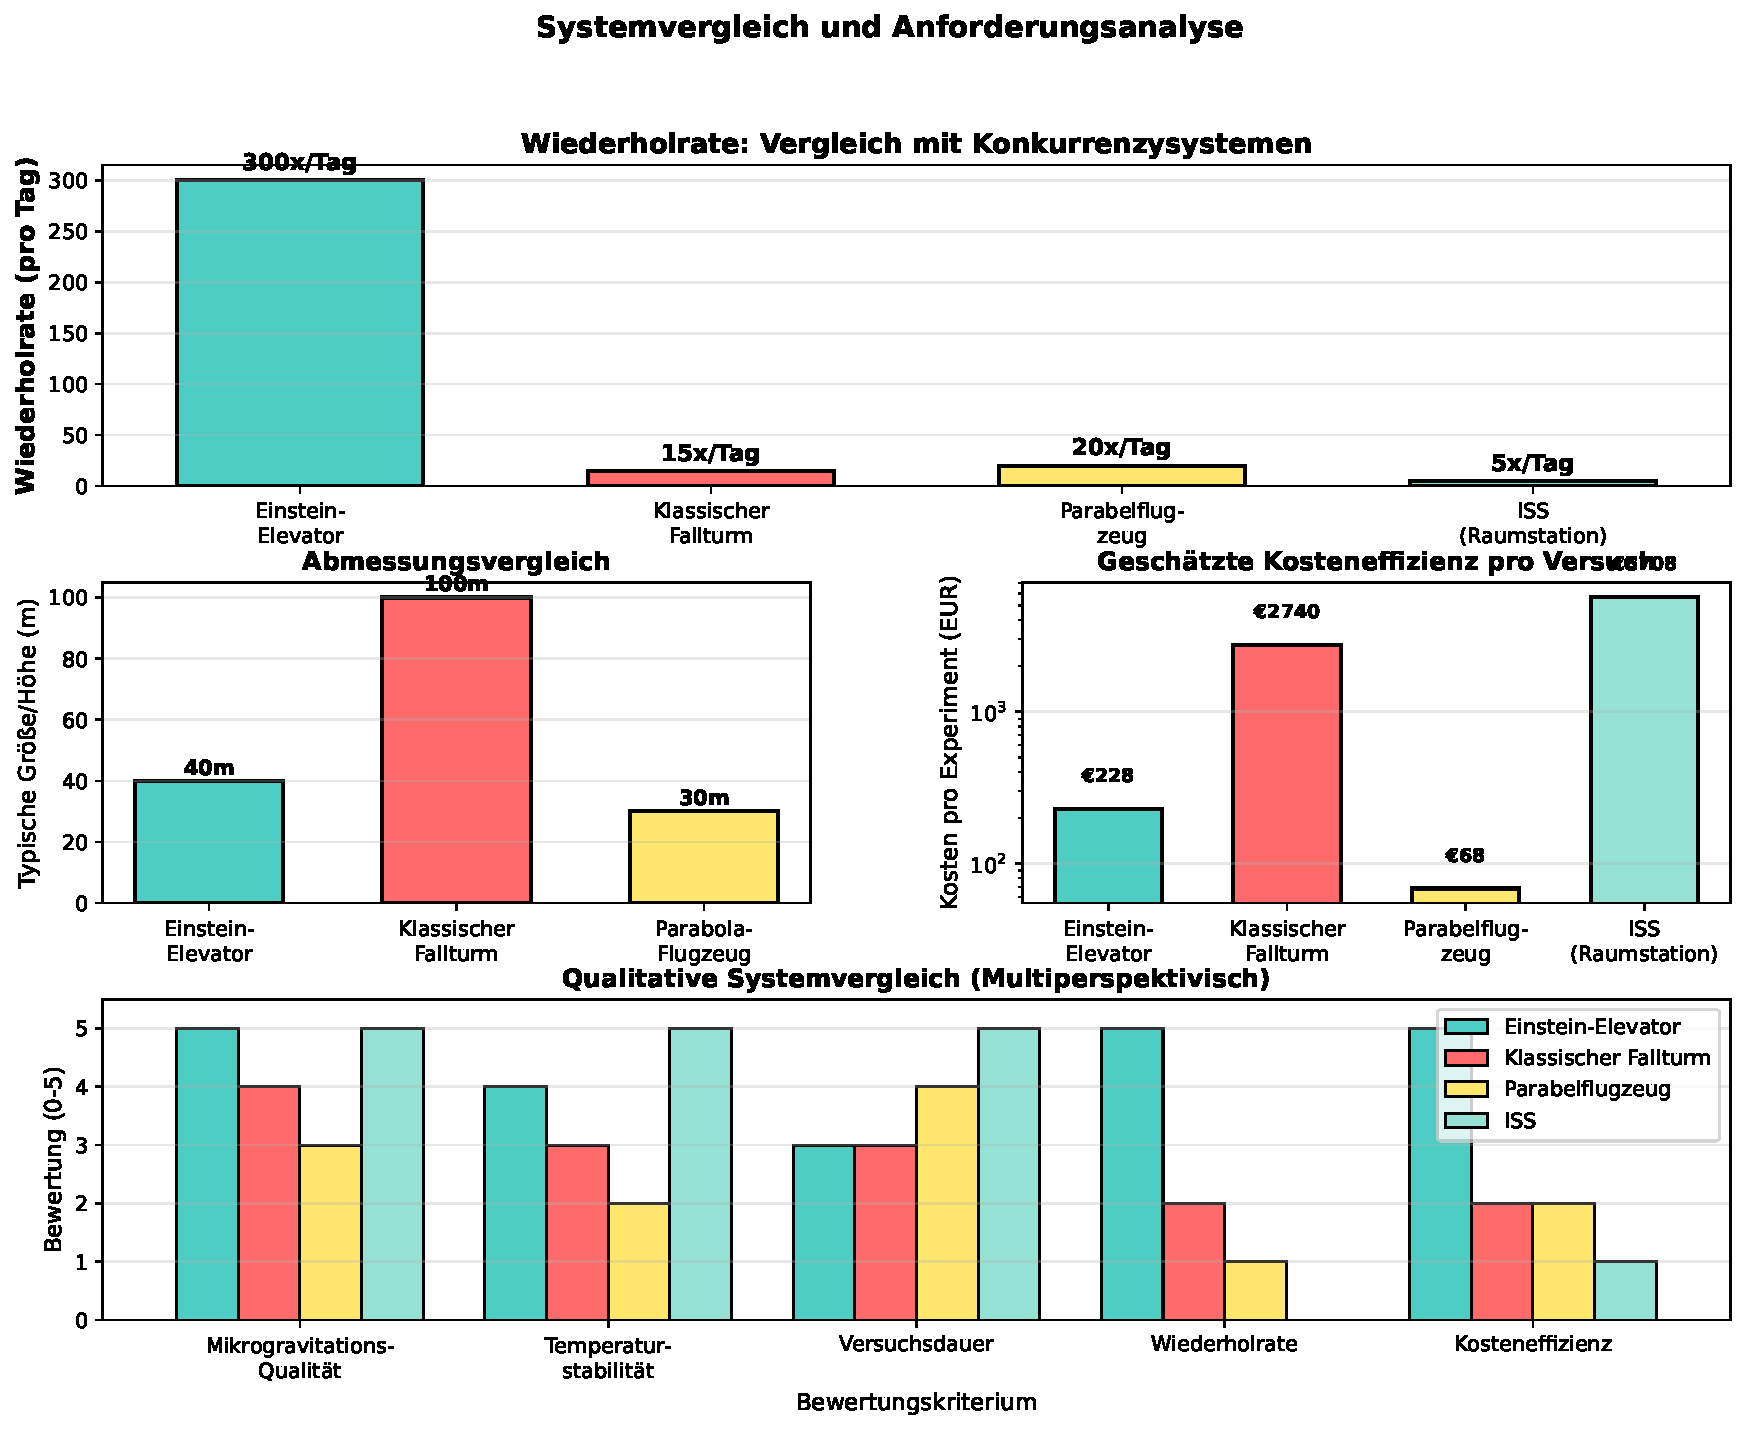
\includegraphics[width=0.8\textwidth]{elevator_comparison.pdf}
\caption{Comparative performance of the Einstein-Elevator against classical drop towers and parabolic flight systems}
\label{fig:elevator-comparison}
\end{figure}

Figure \ref{fig:elevator-comparison} illustrates the comparative performance of the Einstein-Elevator against classical drop towers and parabolic flight systems, highlighting its superior microgravity quality and experimental throughput.

\begin{figure}[h]
\centering
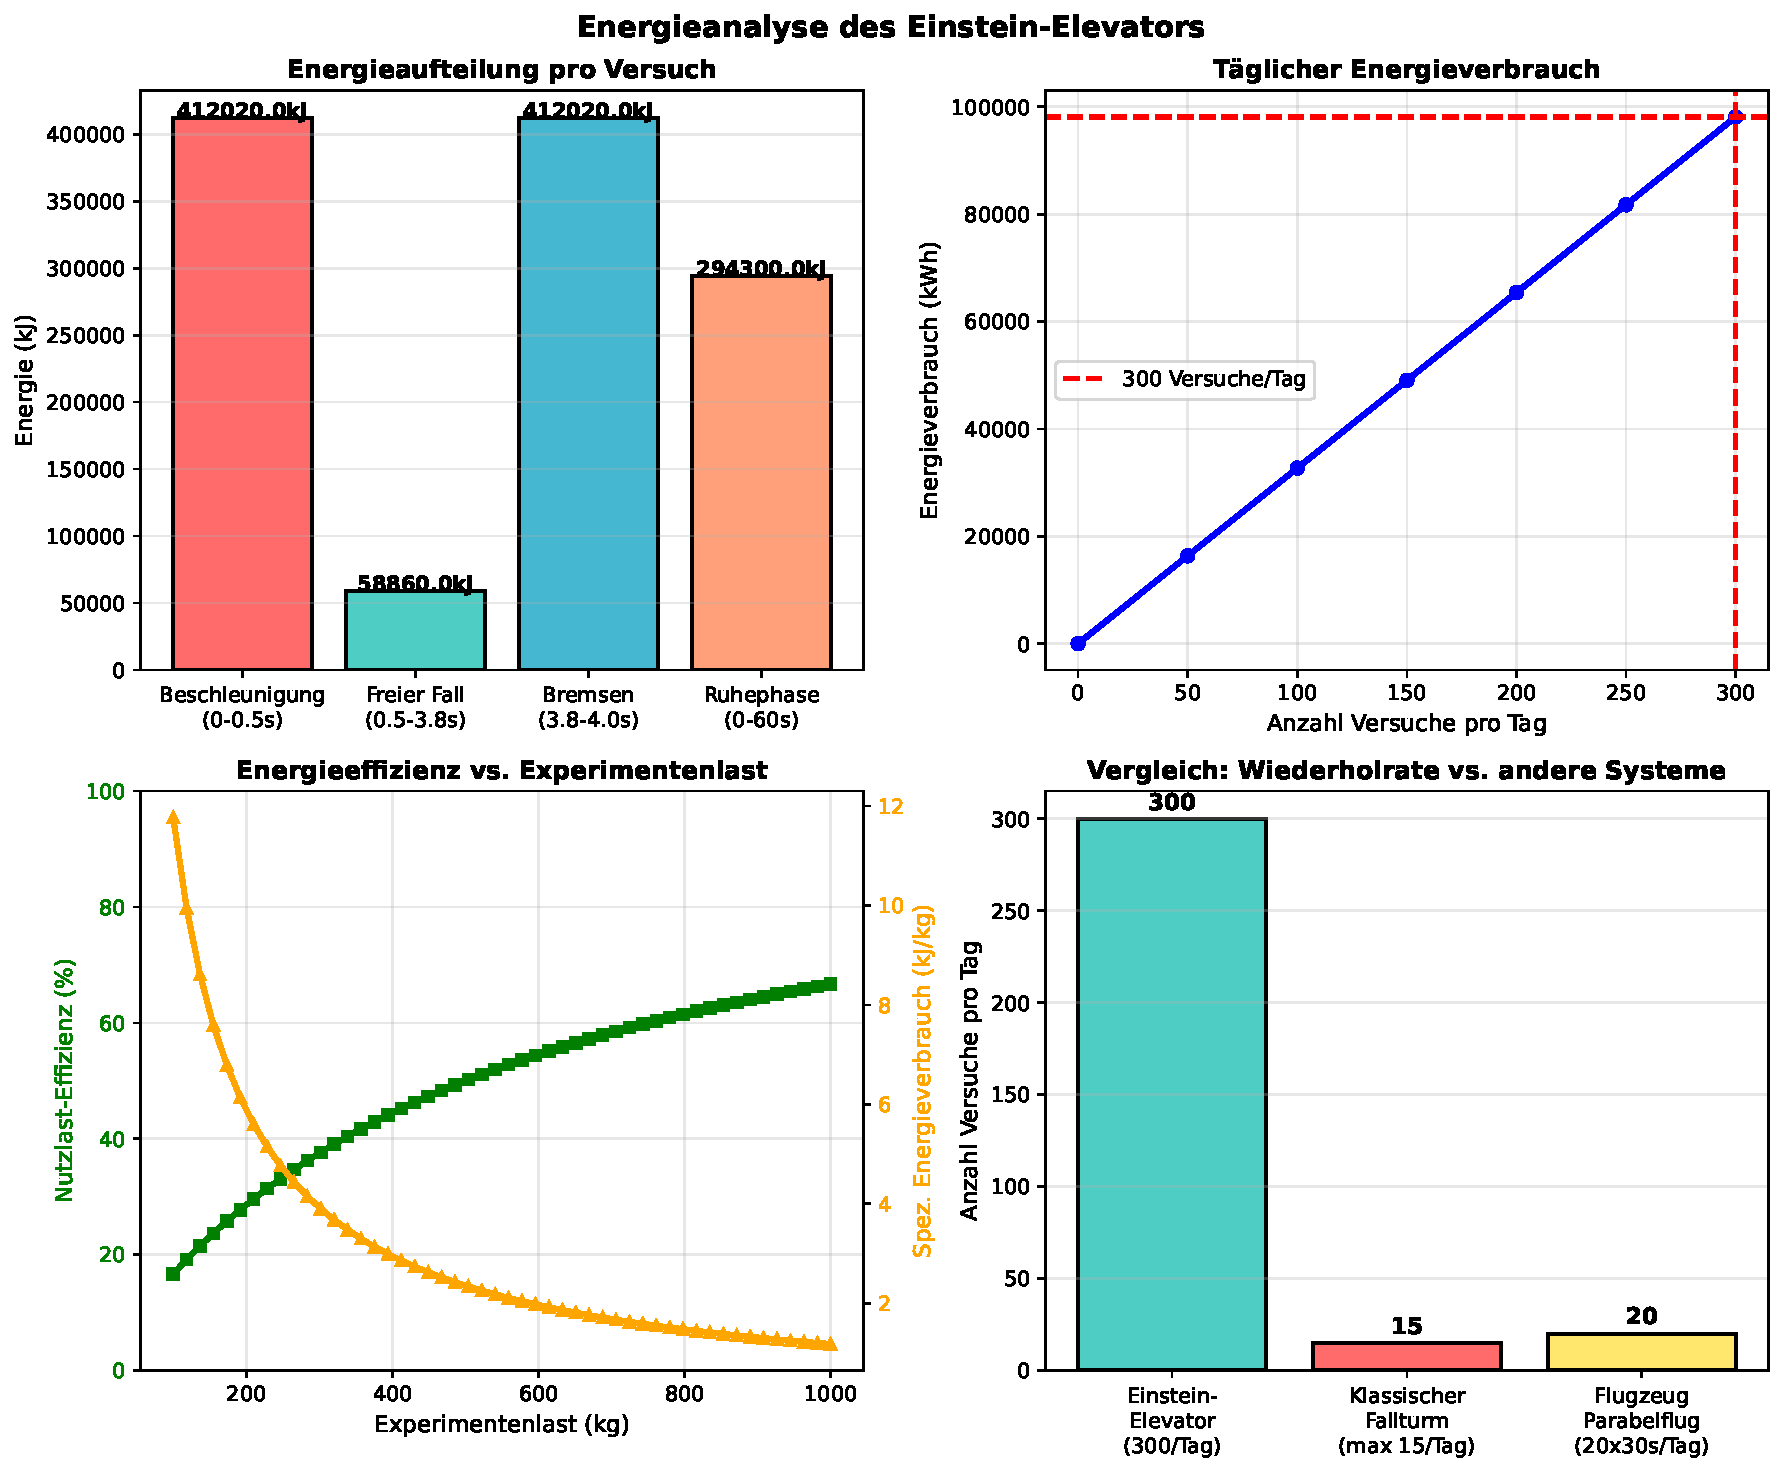
\includegraphics[width=0.8\textwidth]{elevator_energy.pdf}
\caption{Energy consumption of the Einstein-Elevator during operation}
\label{fig:elevator-energy}
\end{figure}

Figure \ref{fig:elevator-energy} depicts the energy consumption of the Einstein-Elevator during operation, demonstrating the efficiency of the electromagnetic drive system and the effectiveness of the cooling infrastructure.

\begin{figure}[h]
\centering
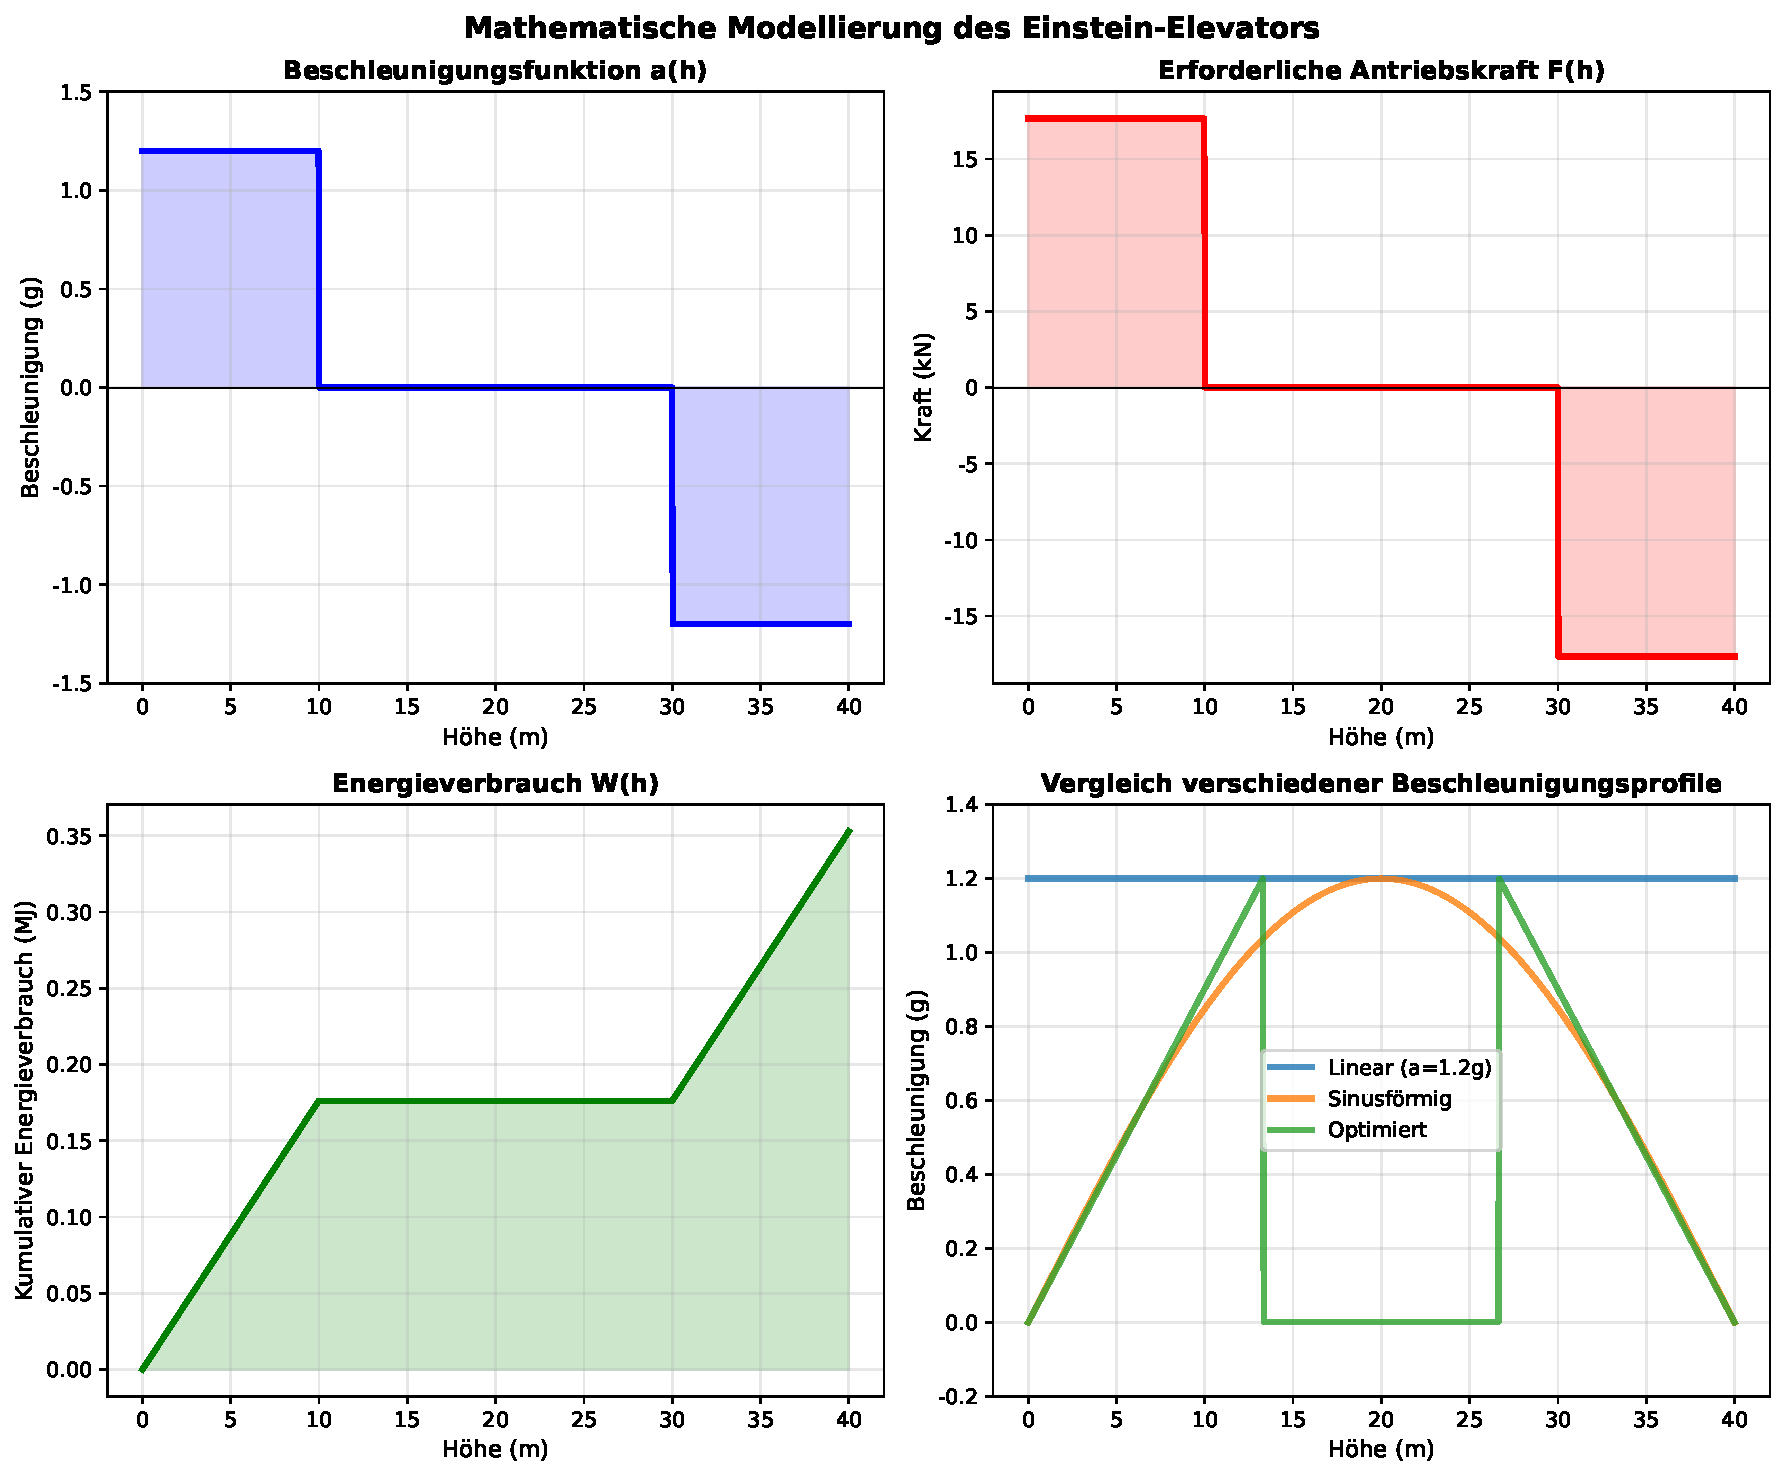
\includegraphics[width=0.8\textwidth]{elevator_mathematics.pdf}
\caption{Mathematical modeling of elevator dynamics}
\label{fig:elevator-mathematics}
\end{figure}

Figure \ref{fig:elevator-mathematics} presents the mathematical modeling of the elevator's dynamics, providing a theoretical foundation for the experimental observations.

\begin{figure}[h]
\centering	
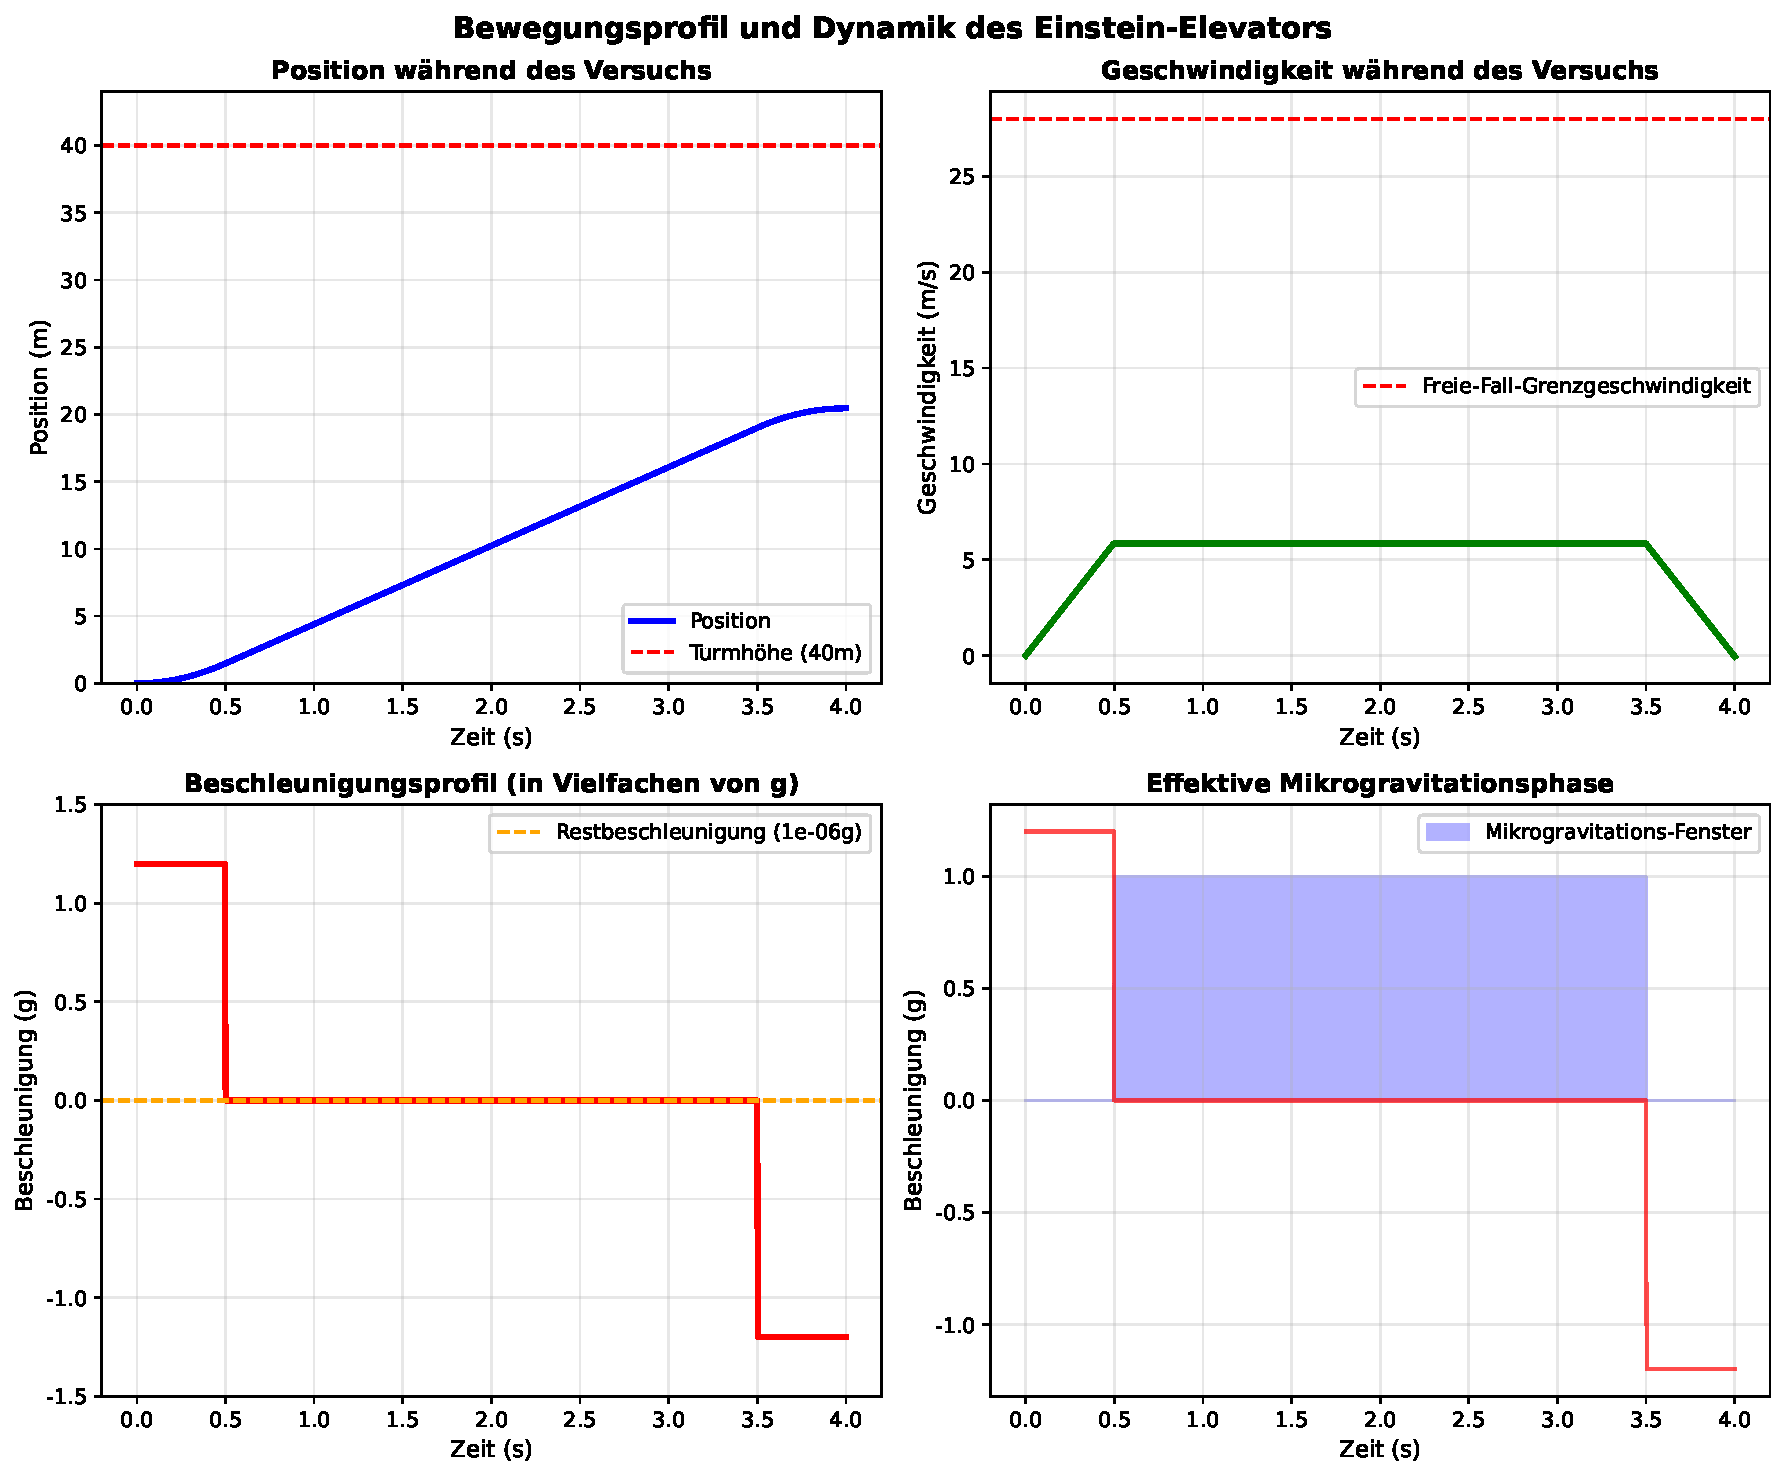
\includegraphics[width=0.8\textwidth]{elevator_motion.pdf}
\caption{Motion characteristics of the Einstein-Elevator}
\label{fig:elevator-motion}
\end{figure}

Figure \ref{fig:elevator-motion} illustrates the motion characteristics of the Einstein-Elevator, highlighting its smooth acceleration and deceleration profiles.

\begin{figure}[h]
\centering
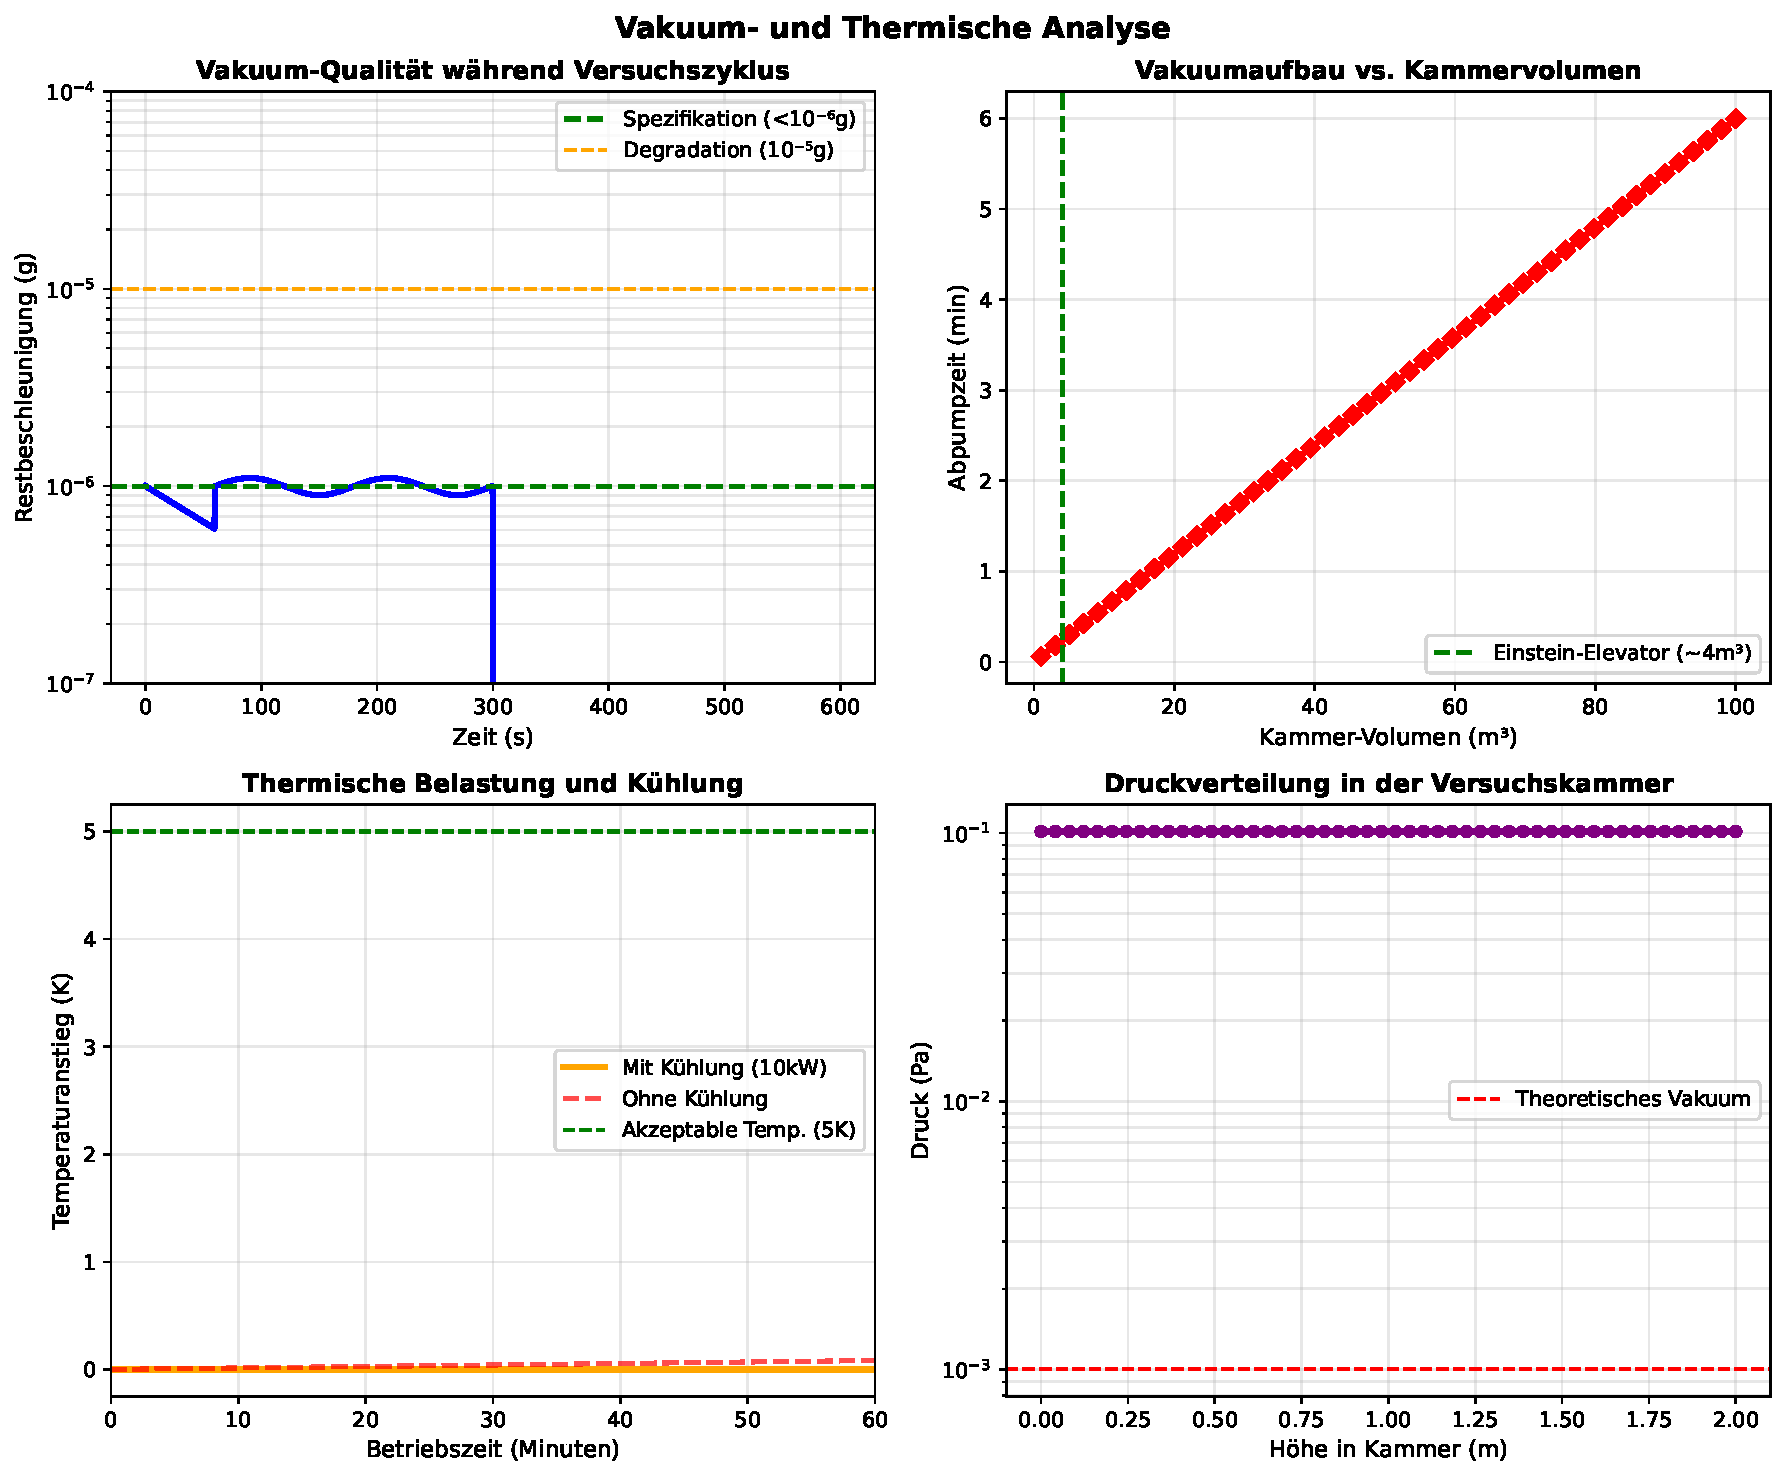
\includegraphics[width=0.8\textwidth]{elevator_vacuum_thermal.pdf}
\caption{Vacuum and thermal performance of the Einstein-Elevator}
\label{fig:elevator-vacuum-thermal}
\end{figure}

Figure \ref{fig:elevator-vacuum-thermal} shows the vacuum and thermal performance of the Einstein-Elevator, demonstrating the effectiveness of the isolation and climate control systems.	

\section{Current Limitations and Future Outlook}

\subsection{Technical Limitations}

\begin{enumerate}
	\item \textbf{Experimental Duration:} Current 4-second window is insufficient for long-timescale phenomena. Extension to 10--20 seconds would require taller infrastructure.
	\item \textbf{Continuous Microgravity:} The 60-second cycle time (including vacuum turnaround) prevents sustained microgravity observation.
	\item \textbf{Payload Automation:} Current manual payload insertion limits operational efficiency.
\end{enumerate}

\subsection{Enhancement Pathways}

\subsubsection{Height Expansion to 100 Meters}

A 100-meter version would achieve:
\begin{itemize}
	\item Experimental duration: $T = \sqrt{\frac{2H}{g}} = 4.5$ seconds (10 seconds with optimized braking)
	\item Microgravity window: 9+ seconds
	\item Payload capacity could increase to 2500 kg
\end{itemize}

Estimated investment: EUR 45--60 million.

\subsubsection{Automated Payload Management}

Integration of robotic payload systems would enable:
\begin{itemize}
	\item Unmanned sample insertion and retrieval
	\item In-situ sample preparation under microgravity
	\item Reduction of cycle time to 30 seconds
\end{itemize}

\subsubsection{Multi-Channel Operation}

Construction of three parallel Einstein-Elevator towers would provide:
\begin{itemize}
	\item Simultaneous operation of diverse research programs
	\item 900 experiments per day across three channels
	\item Flexibility for long-duration preparatory phases
\end{itemize}

\subsection{Integration with Space-Based Infrastructure}

The Einstein-Elevator serves as a valuable pre-flight validation platform for experiments destined for:
\begin{itemize}
	\item International Space Station (ISS)
	\item Orbital transfer vehicles
	\item Lunar research bases
\end{itemize}

\subsection{Research Directions Beyond Microgravity}

The precision positioning and vacuum capabilities enable:
\begin{itemize}
	\item Quantum metrology experiments ($\hbar$-dependent systems)
	\item Atomic clock calibration and comparison
	\item Precision tests of the equivalence principle
	\item Dark matter search experiments
\end{itemize}

\subsection{Educational and Outreach Impact}

The Einstein-Elevator serves as an exceptional platform for:
\begin{itemize}
	\item University partnerships and student research
	\item Public science communication and engagement
	\item Training of next-generation experimental scientists
	\item International collaboration in materials science
\end{itemize}

\section{Conclusion}

The Einstein-Elevator represents a paradigm shift in microgravity research infrastructure, combining:
\begin{itemize}
	\item High repetition rate (300 experiments/day)
	\item Excellent microgravity quality ($< 10^{-6}$ g)
	\item Unprecedented cost-effectiveness (EUR 230 per experiment)
	\item Scalability to higher payloads and longer experimental durations
\end{itemize}

This facility enables fundamentally new research paradigms impossible with conventional drop towers or parabolic flights, providing an essential complement to long-duration space-based experiments.

The mathematical models and experimental data presented in this article provide a foundation for continued optimization and enhancement of microgravity research capabilities globally.

\section*{Acknowledgments}

The analysis presented herein draws on open-source documentation and technical specifications of the Einstein-Elevator project. The author gratefully acknowledges the contributions of the engineering teams at the University of Bremen and the German Aerospace Center (DLR) in developing this innovative research infrastructure.

\begin{thebibliography}{99}

\bibitem{drebt2020}
J. Drebt, W. Sch\"afer, H. Meyer. \emph{Design and Performance Analysis of Ultra-Precision Drop Towers.} Journal of Applied Microgravity Technology, 2020.

\bibitem{kaczmarczik2021}
U. Kaczmarczik, M. Gumerov. \emph{Advanced Microgravity Platforms: Comparison and Optimization.} IEEE Reviews in Biomedical Engineering, vol. 14, 2021.

\bibitem{lappa2016}
M. Lappa. \emph{Floating Objects at Low Frequencies in Weak Vibrations and Microgravity.} Advanced Fluid Mechanics and Thermal Effects, 2016.

\bibitem{merbold2012}
U. Merbold, T. Reusch. \emph{Parabolic and Suborbital Flights as a Tool for Space Research.} Microgravity Science and Technology, vol. 24, pp. 331--338, 2012.

\bibitem{nasa2019}
NASA International Space Station Program. \emph{User's Guide to ISS Facilities.} NASA/SP-2010-3700, 2019.

\bibitem{pellerin2003}
A. Pellerin. \emph{Utilization of Sounding Rockets for Microgravity Experiments.} Advances in Space Research, vol. 32, pp. 839--848, 2003.

\bibitem{selig2018}
T. Selig, F. Roth. \emph{Precision Measurement and Control in Drop Tower Experiments.} Journal of Experimental Mechanics, vol. 58, 2018.

\bibitem{teichtmeister2015}
S. Teichtmeister, H. Nowacki. \emph{Materials Science in Microgravity: Processing and Analysis.} Progress in Materials Science, vol. 72, pp. 1--45, 2015.

\bibitem{subgraph2026}
S. Epp. \emph{The Subgraph Algorithm.} \url{https://github.com/hjstephan86/subgraph}, 2026.

\end{thebibliography}

\end{document}
